\section{The chain skeleton}\label{sec:chain}
Let $u_1,u_2,u_3,u_4$ be the branch vertices in path order. Write $L_{12},L_{23},L_{34}\ge1$ for their original connector lengths. By Lemma~\ref{lem:reduction}, the two terminals may be assumed irreducible. Every central-path edge will point from $u_2$ toward $u_3$.

\subsection{Four half-tree inequalities}
The following inequalities account for the weights in the internal catalogue; all factors in each product are evaluated at the same root label.
\begin{lemma}\label{lem:halftree}
For nonnegative functions $C,F,G$,
\begin{align}
 \Nplus{CTF}&\le\sqrt{\E[qC^4]\,\E[pF^4]},\label{eq:mergeRleft}\\
 \Nminus{CTF}&\le\sqrt{\E[q^5C^4]\,\E[pF^4]},\label{eq:mergeSright}\\
 \Nminus{CAG}&\le\sqrt{\E[pC^4]\,\E[qG^4]},\label{eq:mergeRright}\\
 \Nplus{CAG}&\le\sqrt{\E[p^5C^4]\,\E[qG^4]}.\label{eq:mergeSleft}
\end{align}
\end{lemma}
\begin{proof}
Row Cauchy--Schwarz gives $(TF)^2\le qT(F^2)$. Hence
\[
 \Nplus{CTF}\le\E[pqC^2T(F^2)]\le\E[C^2T(F^2)].
\]
The edge measure for $T$ has root marginal $q\mu$ and other marginal $p\mu$. Cauchy--Schwarz on that measure proves \eqref{eq:mergeRleft}. For \eqref{eq:mergeSright}, retain the extra factors:
\[
 \Nminus{CTF}\le\E[q^2C^2T(F^2)]
 \le\sqrt{\E[q(q^2C^2)^2]\,\E[pF^4]}.
\]
The first term is exactly $\E[q^5C^4]$. Complete reversal gives \eqref{eq:mergeRright} and \eqref{eq:mergeSleft}.
\end{proof}

The merger converts fourth moments into the second moments required by Lemma~\ref{lem:connector}.

\subsection{Compatible directions for all four role combinations}
At the left terminal set $n_1=L_{12}-1$ and use Theorem~\ref{thm:terminal} to define
\[
 G_1^+=T^{n_1}F^+_{1,n_1},\qquad
 G_1^-=A^{n_1}F^-_{1,n_1}.
\]
Then $\E[p(G_1^+)^4]\le1$ and $\E[q(G_1^-)^4]\le1$. Use $n_4=L_{34}-1$ at the right terminal to obtain $G_4^\pm$ with the same bounds. The superscript at a terminal is chosen according to its adjacent internal role in the following table.

\begin{table}[htbp]
\centering
\caption{Compatible outer directions and half-tree bounds.}\label{tab:roles}
\fontsize{9}{11}\selectfont
\setlength{\tabcolsep}{2pt}\noindent\begin{tabular}{@{}p{15mm}p{26mm}p{32mm}p{39mm}p{36mm}@{}}
\toprule
Role & Side message & Entire outer path & Half-tree message & Required output\\\midrule
Left R & $V_2^-$ & $u_1\to u_2$ & $H_\ell=V_2^-TG_1^+$ & $N_+(H_\ell)\le1$\\
Left S & $C_2^-$ & $u_2\to u_1$ & $H_\ell=C_2^-AG_1^-$ & $N_+(H_\ell)\le1$\\
Right R & $V_3^+$ & $u_3\to u_4$ & $H_r=V_3^+AG_4^-$ & $N_-(H_r)\le1$\\
Right S & $C_3^+$ & $u_4\to u_3$ & $H_r=C_3^+TG_4^+$ & $N_-(H_r)\le1$\\
\bottomrule
\end{tabular}

\end{table}

For example, a left type-R vertex has side message $V_2^-$ with $q$-weighted fourth moment at most one. The retained incoming edge contributes $T$, so \eqref{eq:mergeRleft} gives $N_+(H_\ell)\le1$. A left type-S vertex has the fully reversed side message $C_2^-$ with $p^5$-weighted fourth moment at most one; \eqref{eq:mergeSleft} gives the same $N_+$ output, using an outgoing outer path. The right type-R and type-S cases follow from \eqref{eq:mergeRright} and \eqref{eq:mergeSright}, respectively.

The factor $TG$ or $AG$ integrates the final edge of the outer connector; its preceding $L-1$ edges are integrated in $G$. For an outer connector of length one, $G$ is the zero-step terminal message.

The two side tables and the two terminal arm systems are disjoint, so their directions can be chosen independently. For each of the four role combinations RR, RS, SR and SS, the left half produces an $N_+$ bound and the right half an $N_-$ bound.

\begin{figure}[htbp]\centering
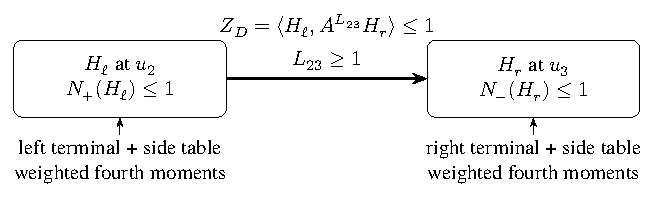
\includegraphics{figures/chain-merger.pdf}
\caption{The chain merger. Terminal and side-table fourth moments give the two indicated half-tree bounds. The outer directions depend on the R/S roles in Table~\ref{tab:roles}; the central connector always points from $u_2$ to $u_3$.}\label{fig:chain}
\end{figure}

\subsection{The complete central path}
After integration over every arm and both outer connector interiors, the original density is exactly
\begin{equation}\label{eq:chaindensity}
 Z_D(K,\mu)=\ip{H_\ell}{A^{L_{23}}H_r}.
\end{equation}
Lemma~\ref{lem:connector} gives
\[
 Z_D(K,\mu)\le\sqrt{N_+(H_\ell)N_-(H_r)}\le1.
\]
Together with the reducible-terminal case, this proves the theorem for the entire $P_4$ skeleton.
